\documentclass[a4paper,10pt]{article}
%\documentclass[a4paper,10pt]{scrartcl}

\usepackage[utf8]{inputenc}
\usepackage[german]{babel}
\usepackage[pdftex]{graphicx}
\usepackage{listings}
\usepackage{color}
\usepackage{amssymb}
\usepackage{marvosym}
\usepackage{amsmath}
\usepackage{array}
\usepackage{geometry}
\usepackage{listings}
\usepackage{upgreek}
\usepackage{color}
\usepackage{gensymb}

\geometry{verbose,tmargin=2cm,bmargin=2cm,lmargin=2cm,rmargin=2.5cm,headheight=80pt}
\newcolumntype{L}[1]{>{\raggedright\arraybackslash}p{#1}} % linksbündig mit Breitenangabe
\newcolumntype{C}[1]{>{\centering\arraybackslash}p{#1}} % zentriert mit Breitenangabe
\newcolumntype{R}[1]{>{\raggedleft\arraybackslash}p{#1}} % rechtsbündig mit Breitenangabe
\newcommand{\tabitem}{~~\llap{\textbullet}~~}

\newcommand{\f}{\noindent\textbf}
\newcommand{\ku}{\textit}
\newcommand{\zb}{z.B.\ }
\newcommand{\ia}{i.A.\ }
\newcommand{\ua}{u.a.\ }
\newcommand{\idr}{i.d.R.\ }

\title{SSD}
\author{}
\date{}

\pdfinfo{%
  /Title    ()
  /Author   ()
  /Creator  ()
  /Producer ()
  /Subject  ()
  /Keywords ()
}

\begin{document}
\maketitle

\section{Spacecraft System Design}
\f{Mission concept:} 
\begin{itemize}
 \item subject (what for)
 \item orbit and constellation
 \item payload, bus
 \item launch element
 \item ground element
 \item mission operations
 \item command, communication, control
\end{itemize}
\begin{figure}[ht!]
 \centering
 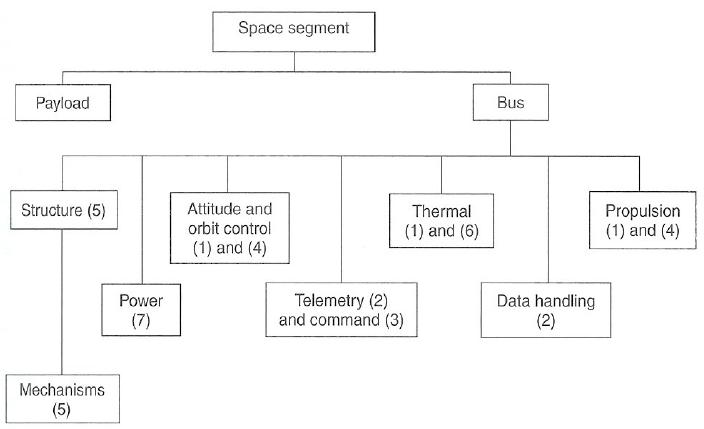
\includegraphics[scale=0.6]{overview}
\end{figure}
\section{Space Dynamics/Kepler Orbits}
\f{Typical coordinate systems:}
\begin{itemize}
 \item spacecraft-fixed
 \begin{itemize}
  \item Mittelpunkt des Satelliten = Ursprung
  \item nadir = z-Achse, nominale Geschwindigkeit = x-Achse
  \item gut, um Position und Orientierung der Satelliteninstrumente festzustellen
 \end{itemize}
 \item earth-fixed 
 \begin{itemize}
  \item Mittelpunkt der Erde = Ursprung
  \item durch greenwich meridian = x-Achse
  \item Geolocation, Satellitenbewegung
 \end{itemize}
 \item roll, pitch and yaw-coordinates 
 \item celestial coordinates
 \begin{itemize}
  \item Mittelpunkt der Erde = Ursprung
  \item Richtung Frühlingspunkt = x-Achse
  \item Orbitanalyse, Astronomie
 \end{itemize}
\end{itemize}
\f{Keplergesetze}
\begin{enumerate}
 \item der Orbit eines jeden Planeten ist eine Ellipse, wobei die Sonne in einem der Fixpunkte liegt
 \item die Verbindungslinie zwischen Sonne und Planet überstreicht in gleichen Zeiten gleiche Flächen 
 \item die Quadrate der Umlaufzeiten sind proportional zu den Kuben der großen Halbachsen
\end{enumerate}
\f{Ellipsendinge}
\begin{itemize}
 \item a \dots große Halbachse
 \item $\varepsilon$, e \dots Exzentrizität, ``Abplattung'' der Ellipse ($\varepsilon$=0: Kreis, $\varepsilon$=1: Parabel, $0<\varepsilon<1$: Ellipse)
\end{itemize}
\f{Begriffe: }
\begin{itemize}
 \item Periapsis: Punkt der Ellipse, der am nähesten an dem Zentralkörper liegt (bei Sonne: Perihel, bei Erde: Perigäum)
 \item Apoapsis: Punkt der Ellipse, der am weitesten entfernt vom Zentralkörper liegt (bei Sonne: Apohel, bei Erde: Apogäum)
 \item Distanz zu Periapsis $r_p = a(1-\varepsilon)$, Distanz zu Apoapsis $r_a = a(1+\varepsilon)$
\end{itemize}
\f{6 Bahnelemente:}
\vspace*{10pt}

\begin{figure}[!ht]
\begin{minipage}{0.35\textwidth}
 \begin{itemize}
  \item große Halbachse a
  \item Exzentrizität $\varepsilon$
  \item inclination i
  \item right ascension of the ascending node $\Omega$
  \item argument of perigee $\omega$
  \item true anomaly $\nu$
 \end{itemize} 
\end{minipage}
\hfill
\begin{minipage}{0.64\textwidth}
  \centering
  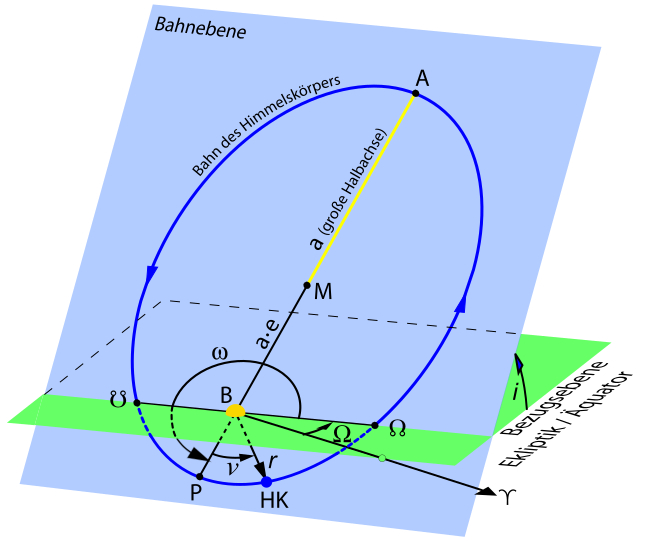
\includegraphics[scale=0.55]{BahnelementeEllipse}
\end{minipage}
\end{figure}
\noindent \f{Lieblingsformel}
\[T = 2\pi\sqrt{\frac{a^3}{\mu}}\]
\f{Change of the right ascension of the ascending node}
\[\Delta \Omega = - \frac{3\pi J_2R_E^2}{a^2(1-\varepsilon^2)^2}cos(i)\]
\f{Change of the argument of perigee}
\[\Delta \omega = \frac{3\pi J_2R_E^2}{2a^2(1-\varepsilon^2)^2}(4-5sin^2(i))\]

\noindent \f{Orbits}
\begin{enumerate}
 \item Highly Elliptical Orbit HEO
 \begin{itemize}
  \item hohe Exzentrizität
  \item große Halbachsen
  \item dadurch lange Kontakdauer zum Satelliten
  \item Werte für Perigäum: 200 bis 15.000 km
  \item Werte für Apogäum: 50.000 bis 140.000 km
  \item für Forschung (\zb Weltraumteleskope), Telekommunikation, Militär 
  \item Beispiel: Molniya-Orbit (feste Inklination von 63,4$^\circ$, Periodendauer von einem halben Sterntag (23h56m4s))
 \end{itemize}
 \item Sun-Synchronous Orbit
 \begin{figure}[!ht]
  \centering
  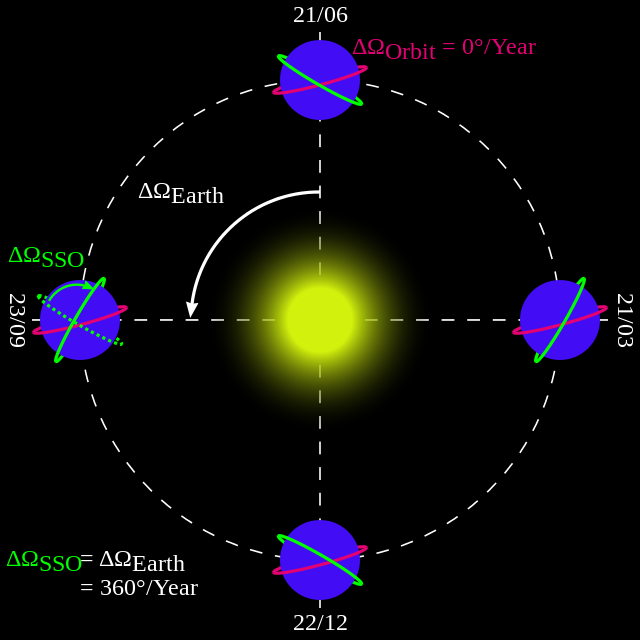
\includegraphics[scale=0.4]{sso}
 \end{figure}
 \begin{itemize}
  \item Höhe und Inklination werden so kombiniert, dass ein Satellite aus Sicht der Sonne immer auf dem selben Orbit ist
  \item Höhe: 600-800 km
  \item Inklination: leicht retrograd ($\approx 98^\circ$)
  \item Umlaufdauer: 96-100min
 \end{itemize}

 \item Geostationary Orbit GEO
 \begin{itemize}
  \item kreisförmiger Orbit
  \item Höhe: 35.786km
  \item Umlaufdauer: 24h
  \item Wettersatelliten, Kommunikationssatelliten, Fernsehsatelliten
 \end{itemize}

\end{enumerate}

\noindent \f{Subsatellite Point} = intersection of the line between satellite and earth center with the earth's surface 
\noindent \f{Hohmann Transfer}
\begin{figure}[!ht]
 \centering
 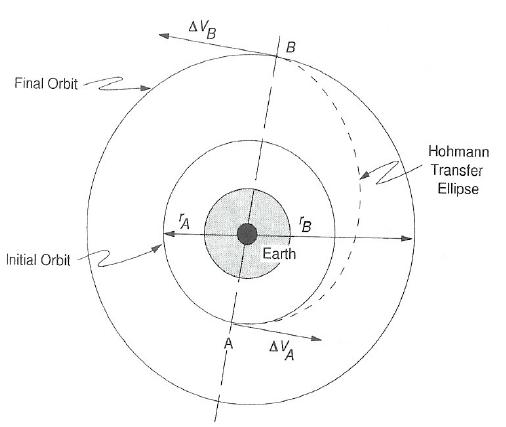
\includegraphics[scale=0.6]{hohmann}
\end{figure}

\begin{itemize}
\item Calculate a transfer between two circular orbits with radius $r_A$ to $r_B$. The velocity at pericenter of the transfer ellipse:
\[ v_P^2 = 2 \mu \left( \frac{1}{r_A} - \frac{1}{r_A + r_B} \right) = 2 \mu \frac{r_B}{r_A(r_A+r_B)} \]
\item The required $\Delta v_A$ to inject from the transfer orbit:
\[ \Delta v_A = v_P - v_A = \sqrt{\frac{\mu}{r_A}} \left( \sqrt{\frac{2r_B}{r_A+r_B}} -1\right) \]
\item The required $\Delta v$ to inject from the transfer orbit into orbit with $r_B$:
\[ \Delta v_B = v_B - v_\text{apo} = \sqrt{\frac{\mu}{r_B}} \left( 1 - \sqrt{\frac{2r_A}{r_A+r_B}}\right) \]
where $v_B$ is the circular velocity at $r_B$.
\item The Hohmann transfer is the most energy-efficient transfer between two circular orbits.
\[ \Delta v_\text{total} =  \Delta v_A + \Delta v_B = \sqrt{\mu}\left[ \sqrt{\left( \frac{2}{r_A} - \frac{2}{r_A+r_B} \right)} - \sqrt{\frac{1}{r_A}} + \sqrt{\frac{2}{r_B}-\frac{2}{r_A+r_B}} - \sqrt{\frac{1}{r_B}} \right]\]
\end{itemize}

\section{Mission Analyses}
\f{Earth-Synchronous Orbit}
\begin{itemize}
 \item the ground track repeats after a specific period of time
 \item Earth's rotation rate is the sidereal rotation period = sidereal day $\uptau_{\text{\tiny{E}}}$
 \item $\uptau_E$ is varying with time $\uptau_E = 86164.10555+0.15\cdot C$ [s] where C is the centuries since year 2000
 \item as the Earth rotates eastward, the satellite is thus moving relative to the surface in westward direction by 
 \[\Delta \Phi_r = 2\pi\frac{T}{\uptau_{\text{\tiny{E}}}} \text{ [rad/rev]}\] 
 \item second effect influencing the shift of the subsatellite point is the rotation of the satellite's orbit plane $\Delta \Omega$
 \item as $\Delta \Omega$ is positive in eastward direction, these two effects are combined to the total angular shift $\Delta \Phi$ at subsequent equator 
 passages \[\Delta \Phi = \Delta \Phi_r - \Delta \Omega \text{ [rad/rev]}\]
 \item to be Earth-Synchronous: 
 \[n\Delta \Phi = m \cdot 2\pi\]
\end{itemize}
\f{Sun-Synchronous Orbit}
\begin{itemize}
 \item die Erde braucht $\uptau_S = 3.155815\cdot 10^7 s$, um einmal um die Sonne zu kreisen 
 \item bei einem sonnensynchronen Orbit muss der Winkel zwischen Sonnenrichtung und Orbitebene konstant bleiben 
 \item also muss sich die Ebene pro Tag um einen Winkel $\theta$ drehen 
 \[\theta = 2\pi\frac{\uptau_{\text{\tiny{E}}}}{\uptau_{\text{\tiny{S}}}} \text{ [rad/day]} = 2\pi\frac{\uptau_{\text{\tiny{E}}}}{\uptau_{\text{\tiny{S}}}}\frac{T}{\uptau_{\text{\tiny{E}}}} \text{ [rad/rev]}\]
\end{itemize}
\f{Earth- and Sun-Synchronous Orbit}
\begin{itemize}
 \item \[\Delta \Omega = \theta \Rightarrow T\left(\frac{1}{\uptau_{\text{\tiny{E}}}} - \frac{1}{\uptau_{\text{\tiny{S}}}}\right) = \frac{m}{n}\]
 \item angular shift between two subsequent orbits 
 \[\Delta \Phi = \Delta \Phi_r - \Delta \Omega = 2\pi T\left(\frac{1}{\uptau_{\text{\tiny{E}}}} - \frac{1}{\uptau_{\text{\tiny{S}}}}\right) \text{ [rad/rev]}\]
 worst case between subsequent orbits $\Delta \Phi \cdot R_E$.
\end{itemize}
\f{Eclipse periods}
angle between Earth-Sun vector and normal vector to orbit plane: $\sin \beta = \vec{s}\cdot\vec{n}$\\
Earth central angular radius at entry into eclipse: $\beta^* = \sin^{-1}\left(\frac{R_E}{h+R_E}\right)$\\
Angular arc of orbit in shadow: $2\cos^{-1}\left(\frac{\cos \beta^*}{\cos \beta}\right)$
\f{Ground Contact and Coverage Analyses}
altitude $h$, visible horizon characterized by angles $\rho$ and $\lambda_0$: $\rho + \lambda_0 = 90\degree$
\begin{align*}
 R_E &= (R_E + h) \cos \lambda_0\\
 &= (R_E +h) \sin \rho\\
\end{align*}
observe $\Lambda_t, \Theta_t$ (long,lat) from known orbit position of satellite, characterized by subsatellite point $\Lambda_s, \Theta_s$.\\
characteristic paramters:
\begin{itemize}
 \item nadir angle $\eta$
 \item earth central angle $\lambda$
 \item spacecraft elevation angle $\varepsilon$
\end{itemize}
\begin{figure}[!ht]
 \centering
 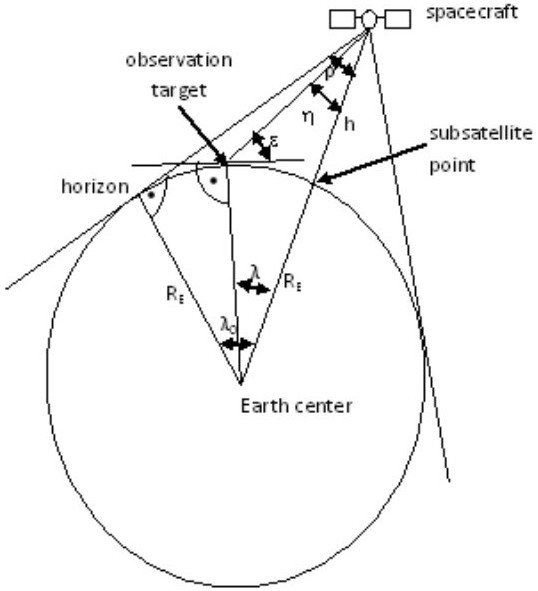
\includegraphics[scale=0.6]{groundcoverage}
\end{figure}
calculate nadir angle $\eta$:
\[ \tan \eta = \frac{\frac{R_E}{R_E+h}\sin \lambda}{1-\frac{R_E}{R_E+h}\cos\lambda}\]
\[ \lambda + \eta + \varepsilon = 90\degree \]
$\lambda_\text{max}$: maximum earth central angle $\Rightarrow$ swath width $2\lambda_\text{max}$ perpendicular to groundtrack on surface.\\
Time in view $T_\text{view}$ for circular orbit with period $T$:
\[ T_\text{view} = \frac{T}{180\degree}\cos^{-1}\left(\frac{\cos \lambda_\text{max}}{\cos \lambda}\right)\]
\f{ground station contact periods}
\begin{figure}[!ht]
 \centering
 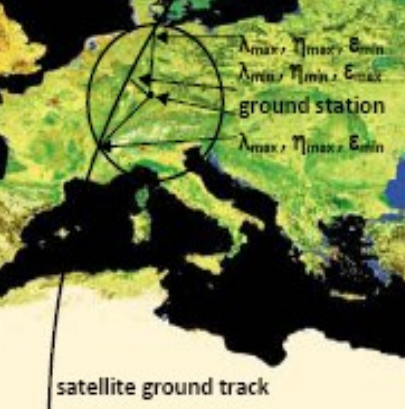
\includegraphics[scale=0.6]{groundtrack}
\end{figure}
\begin{itemize}
 \item $\sin\eta_\text{max} = \cos \varepsilon_\text{min}\frac{R_E}{R_E+h}$
 \item $\lambda_\text{max} = 90\degree - \varepsilon_\text{min} -\eta_\text{max}$
 \item max range satellite$\leftrightarrow$groundstation: $D_\text{max} = R_E\frac{\sin\lambda_\text{max}}{\sin\eta_\text{max}}$
 \item total time in view: $ T_\text{view} = \frac{T}{180\degree}\cos^{-1}\left(\frac{\cos \lambda_\text{max}}{\cos \lambda_\text{min}}\right)$
 \item contact only possible, if station-orbit angle $<$ central angle of contact cone
\end{itemize}


\section{Distributed Satellite Systems}
\begin{itemize}
 \item \f{constellation}: similar trajectories without relative position control.
 \item \f{formation}: closed-loop onboard control for topology in the group.
 \item \f{swarm}: similar vehicles cooperating without fixed positions, selfdetermined.
 \item \f{cluster}: heterogenous system of vehicles for joint objective.
\end{itemize}
requirements on distributed satellite systems: coordination of
\begin{itemize}
 \item orbits at different altitudes
 \item optimal control strategies for position/attitude of components
 \item activities for heterogenous sensors
 \item information flow and storage
\end{itemize}
\f{Walker Delta Pattern Constellation}
\[ i: t/p/f \]
\begin{itemize}
 \item i: inclination
 \item t: total $\sharp$ satellites
 \item p: $\sharp$ equally shaped orbit planes
 \item f: relative phase difference between satellites in adjacent planes
\end{itemize}
Example: Galileo is $56\degree: 27/3/1$ with circular orbits ($h =23222km$), nine satellites always in view, one spare satellite in each plane.
\f{earth surface converage}
$ s = \frac{t}{p}$ number of satellites equally spaced in plane with angular distance $\Delta v = \frac{360\degree}{s}$. There are two cases:
\begin{itemize}
 \item $\Delta v < 2\cdot \lambda_\text{max} \Rightarrow$ area of continuous coverage exists (``street of coverage'')
 \item $\Delta v > 2\cdot \lambda_\text{max} \Rightarrow$ no street of coverage
\end{itemize}
Street-width: $\cos \lambda_\text{street} = \frac{\cos\lambda_\text{max}}{\cos\frac{\Delta v}{2}}$

\f{formation flying arcitectures and dynamics}
\begin{itemize}
 \item \f{virtual structure}: treated as single structure
 \item \f{behavioral strategies}: distributed control approach, following nature.
 \item \f{leader-follower}: divided into leaders and followers. followers track designated leaders with prescribed offset. absolute/relative control architecture.
\end{itemize}

\f{communication in low-earth orbit distributed satellite systems}
\begin{itemize}
 \item comm and tele-operation infrastructure is key element for distributed systems
 \item transfer position and observation data for formation flying
 \item amount of data increases with swarm size
 \item analyse pre-processing procedures, intersatellite links and ground station links
\end{itemize}

\f{conclusion on distributed satellite systems}
\begin{itemize}
 \item research field due to paradigm shift from one large spacecraft to several smaller crafts
 \item higher fault tolerance and robustness
 \item swarms are scaleable
 \item gun launches into orbit
 \item comination of big and small spacecrafts
 \item swarms for survailance and earth observation
 \item LEO $\rightarrow$ high spatial resolution
 \item higher temporal resolution is provided by constellations with several satellites in the same orbit
\end{itemize}

\section{Mechanics}
\f{mechanical system engineering}
\begin{itemize}
 \item \f{mechanical specs}: requirements on satellite, components and equipment
 \item \f{verification plan}: ``how to prove satellite complies specs?'' test, simulations, similarity
 \item \f{test plan}: test flow, model philosophy (QM/FM$\leftrightarrow$PFM)
 \item \f{design loads}: simplified load cases for components \& equipment
\end{itemize}

\f{requirements on satellite structures}\\
\begin{tabular}{ll}
    \tabitem external shape &
    \tabitem mass, center of gravity\\
    \tabitem resonance frequency&
    \tabitem thermo-elastic distortion\\
    \tabitem interfaces&
    \tabitem environment (vacuum, debris, etc.)\\
    \tabitem margin of safety\\
\end{tabular}

\f{random vibration loads}
\begin{itemize}
 \item white noise: range $20-2000Hz$, max levels at $80-300Hz$
 \item mainly acoustic excitation under fairing
 \item depends on location, orientation, mass
 \item equivalent design loads: 3 times root mean square (3 sigma value)
\end{itemize}

\f{shock events}
\begin{itemize}
 \item launcher-induced: stage separation, fairing
 \item S/C release: clampband, discrete pyro devices
 \item appendage release: protechnic/deployment shock
\end{itemize}

\f{structural engineering -- fundamentals}
\begin{itemize}
 \item hooke's law: $\sigma = E\cdot\varepsilon$
 \item strain def: $\varepsilon = \frac{\Delta L}{L}$
 \item normal stress in rod: $\sigma = \frac{F}{A}$
 \item bending stress in beam: $\sigma = \frac{M}{W}$
 \item thermo-elastic strain: $\varepsilon = CTE\cdot \Delta T$
\end{itemize}

\f{Margin of safety:}
\[ MOS = \left(\frac{S_a}{S_e\cdot FOS} -1\right)\cdot 100 \stackrel{!}{\geq} 0,0 ~~~ [\%] \]
\begin{tabular}{lll}
 \tabitem $S_a$ allowable stress &
 \tabitem $S_e$ applied stress &
 \tabitem $FOS$ Factor of safety\\
\end{tabular}

\f{safety factors:}
\begin{itemize}
 \item material safety factors on yield
 \item modelling safety factors covering analysis uncertainties
 \item specific factors, e.g. for bonded connections
\end{itemize}

material selection driven by\\
\begin{tabular}{ll}
 \tabitem ratio stiffness/mass & \tabitem ratio strength/mass\\
 \tabitem functional aspects & \tabitem compability with environment \\
 \tabitem thermoelastic behavior & \tabitem manufacturing complexity \\
 \tabitem sources & \tabitem cost\\
\end{tabular}

\f{test facilities}
\begin{itemize}
 \item electro-dynamic shaker testing orthogonal axes
 \item tasks: system identification -- model correlation -- model adaption
\end{itemize}

notching -- reduction of dynamic loads -- prevents exeeding design limit loads, preventing satellite structure damage.
primary notching -- whole satellite $\leftrightarrow$ secondary notching -- satellite subsystems

\f{tests}
\begin{itemize}
 \item acoustic noise tests
 \item separation tests
\end{itemize}

\f{typical loads:}\\
\begin{tabular}{|l|l|}
\hline
 static & $<10g$ \\
 quasi-static & up to $100g$ \\
 sine & up to $100g $\\
 random & sometimes $>100g$ (3 Sigma)\\
 acoustic noise & ~$100dB$\\
 shock & $2000g$\\
\end{tabular}

\f{critical requirements}
\begin{itemize}
 \item zero grav
 \item launch loads
 \item extreme temperatues
 \item vacuum -- lubrication is critical
 \item no maintainance
\end{itemize}






\section{Thermal Engineering}
\f{general task}
\begin{itemize}
 \item engineering: define requirements and design
 \item analysis: establish thermal mathematical model (TMM), perform distribution calculations
 \item test: plan, perform, evaluate realistic tests
\end{itemize}

\f{satellite thermal control -- requirements}
\begin{itemize}
 \item temperature limits!
 \item temperature gradients, -stability, -uniformity
 \item heatflux, -storage
 \item power and mass-allocation
\end{itemize}

\f{heat mechanisms:}
\begin{itemize}
 \item radiation: transfer via electromagnetic waves
 \item conduction: transfer via fluids and solids in absense of fluid motion
 \item convection: transfer in a flowing fluid and between fluid and wall (mostly irrelevant in satellites)
\end{itemize}

\f{thermo optical properties of materials}
\begin{figure}[ht!]
 \centering
 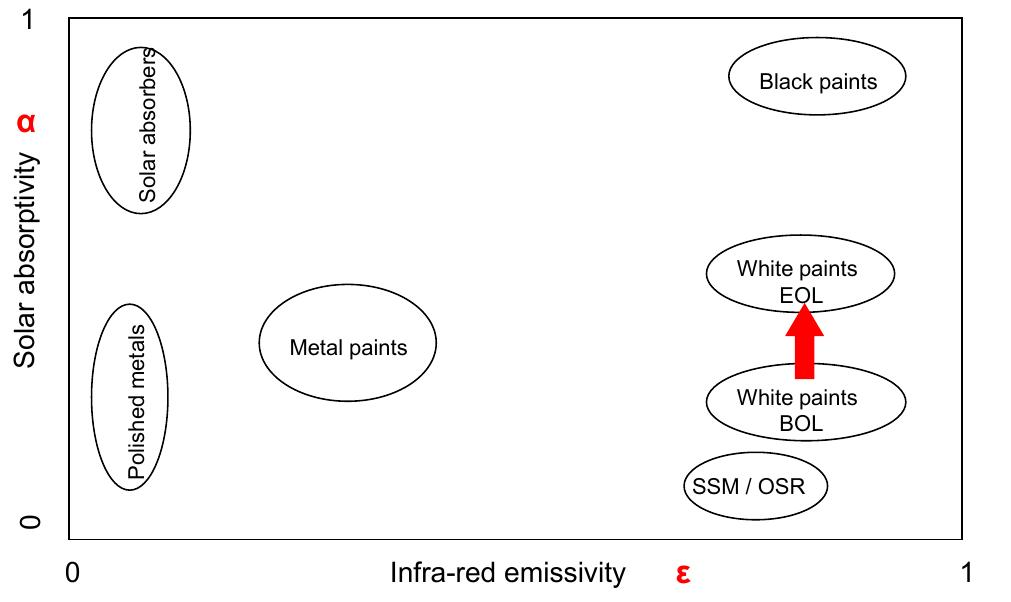
\includegraphics[scale=0.6]{thermooptical}
\end{figure}

\f{global energy balance}\\
\begin{tabular}{ll|ll}
 \tabitem Solar intensity & $\dot{q}_S = 1316\dots1428 \frac{W}{m^2}$ &  \tabitem Earth albedo & $\dot{q}_A = 0.2\dots0.4\dot{q}_S$ \\
 \tabitem Earth IR Radiation & $\dot{q}_E = 189\dots261 \frac{W}{m^2}$ &  \tabitem Absorbtivity Coefficient& $\alpha = 0\dots 1$ \\
 \tabitem Emissivity Coefficient & $\varepsilon = 0\dots 1$ &  \tabitem View Factor & $\phi = 0\dots 1$ \\
\end{tabular}

\f{orbital environment and load cases:}
\begin{itemize}
 \item external loads (sun, earth, moon...)
 \item LEO, GEO, lagrange, eclipse?
 \item orientation (earth, sun, deepspace?)
 \item operating modes
 \item mission scenario
\end{itemize}

\f{typical design load cases}\\
\begin{tabular}{l|l|l}
 & cold case & hot case \\
 \hline
 environment& cold external, BOL& hot external, EOL\\
 solar intensity& min $(\sim1320 \frac{W}{m^2})$ & max $(\sim1420 \frac{W}{m^2})$\\
 earth albedo& min $(\sim0.2)$ & max $(\sim0.4)$\\
 earth IR radiation & min $(\sim200 \frac{W}{m^2})$& max $(\sim260 \frac{W}{m^2})$\\
\end{tabular}

\f{thermal design -- approach}
\begin{itemize}
 \item insulate against environment
 \item minimize absorbed heat
 \item balance internal heat
 \item define radiator-areas and distribute heat
 \item install thermal control hardware
 \item analyze and verify TCS (thermal control system)
\end{itemize}

\f{critical components}
\begin{itemize}
 \item batteries
 \item detectors and sensors (instrument \& star)
 \item optical equipment
 \item mechanisms, tubes, propulsion systems
\end{itemize}

\f{thermal control hardware}
\begin{itemize}
 \item insulation, surface coating
 \item thermal interfillers
 \item thermal doublers, heat straps, heatpipes
 \item electrical heaters, temperature sensors
\end{itemize}






\section{Rocket Propulsion}

\f{Propulsion systems:} \textit{(experimental)}
\begin{itemize}
 \item chemical: solid, liquid, hybrid, \textit{gelled}
 \item electrical: \textit{electo-thermal, electrostatic}, electromagnetic
 \item photonic: \textit{photon, solar sails}
 \item nuclear: \textit{solid core, gas core, nuclear electric}
 \item cold gas thrusters
\end{itemize}

\f{principals}
\begin{itemize}
 \item ejection of mass, provided by onboad means
 \item conservation of momentum, no momentum transfer to external medium
 \item continuous acceleration
\end{itemize}

\f{staged vehicles}
\begin{itemize}
 \item tandem staged
 \item parallel staged
\end{itemize}

\f{liquid Propulsion systems}
\begin{itemize}
 \item pressure feed system: high-pressure gas supply, pressure regulation, most simple and reliable
 \item turbopump feed system: propellant pressurized by pump, driven by turbine, high thrust and long duration
\end{itemize}

\f{selection criteria}
\begin{itemize}
 \item performance: specific impulse, energy release per propellant mass, combustion, ignition, coolant performance
 \item economic: availability, cost, logistics
 \item handle: condition at ambient, non-toxic, non-corrosive, hazards
\end{itemize}

\f{mono-propellants}
\begin{itemize}
 \item energy release by decomposition, stable under controlled environment
 \item ignition: thermally, catalytic
 \item advantages: simple tankage, feeding, flow, injection
 \item e.G.: hydrogen peroxide ($H_2O_2$), hydrazine ($N_2H_4$)
\end{itemize}

\f{bipropellants}
\begin{itemize}
 \item chemical reaction of two propellants ($O_2, H_2$ or $O_2$, kerosene)
 \item separate storage, mixing
 \item high performance, safe operation
 \item \f{hypergolic propellants:} toxic, trained personel required, pollution risk at launch failure
 \item \f{cryogenic propellants:} gaseous at ambient, need thermal insulation, high power
\end{itemize}

\f{combustion}
\begin{itemize}
 \item before chem. reaction, fuel has to atomize/evaporate
 \item mixing of propellants
 \item timescale: chem $\ll$ atomization, evaporation, mixing
 \item temperatur increase $\rightarrow$ gas volume increase $\rightarrow$ velocity increase
 \item chamber cooling: cooling fluids (fuel), film injection, thermal emission
\end{itemize}

\f{ignition}
\begin{itemize}
 \item pyro: solid propellant, electrilly ignited
 \item spark plug: sparks ignite in combustion chamber
 \item spark torch: seperate igniter combustion chamber
 \item laser: beam focused in combustion chamber
\end{itemize}

\f{solid propellants}
\begin{itemize}
 \item long time storage
 \item range of thrust levels: $2N\dots 10MN$
 \item no moving parts, no service
 \item no shutoff, toxic
 \item applications: boosters, upper stage engines, tactical missiles, gas generation
\end{itemize}

\f{electric propulsion}
\begin{itemize}
 \item electrothermal: heating of propellant by contact with hot metal
 \item electrostatic: acceleration of charged particels 
 \item electromagnetic: acceleration of highly ionized plasma
\end{itemize}

\f{launchers}\\
\begin{tabular}{l|clcc}
 & first launch & space ports& LEO & GTO \\
 \hline
 HII (Japan) & 1994 & Tanegashima& 19 T & 4-8 T\\
 Soyuz (Russland)& 1957 & Baikonur/Plesetsk& 6 T& 1.3 T\\
 Ariane 5 (Europa) & 1996& Kourou& -- & 9.6 T \\
\end{tabular}

\section{TT\&C}
\f{terminology}
\begin{itemize}
 \item radiocommunication service RR20 -- involving the transmission/reception of radio waves
 \item frequency allocation RR17 -- entry in the table of frequencies of given band for radiocommunication services
 \item frequency assignment RR18 -- authorisation to use radio frequency under conditions
\end{itemize}

\f{communication delay}
\begin{figure}[ht!]
 \centering
 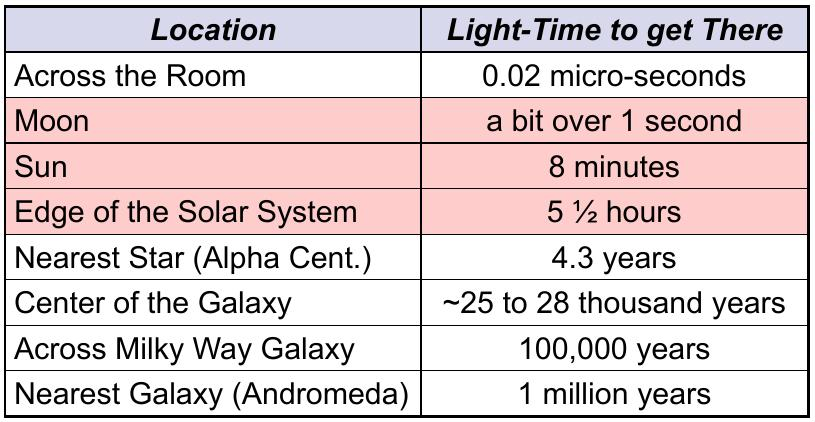
\includegraphics[scale=0.6]{commdelay}
\end{figure}

\f{bands -- frequencies \& wavelength}
\begin{figure}[ht!]
 \centering
 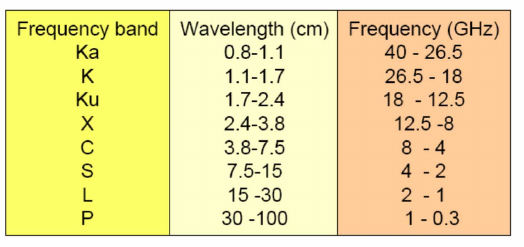
\includegraphics[scale=0.6]{bands}
\end{figure}

\f{band usage}
\begin{itemize}
 \item S: SOHO, XMM-Newton, Cluster, Integral
 \item X: Mars Express, Rosetta, Venus Express, Herschel, Plank
 \item $K_a$: LISA Pathfinder, Gaia, James Webb Space Telescope, BepiColumbo
\end{itemize}

\f{transponder operations}
\begin{itemize}
 \item Uplink Carrier, Carrier + Telecommand, Carrier + TC + Ranging
 \item Downlink Carrier, Carrier + Telemetry, Carrier + TM + Ranging
 \item auto-switch into coherent mode
\end{itemize}

\f{reasons for modulation}
\begin{itemize}
 \item to separate signals
 \item to select correct frequency
 \item easier transmission
\end{itemize}

\f{typical modulation types}
\begin{itemize}
 \item uplink: $2 \frac{kbits}{s}$ bitstream is phase-modulated onto 16kHz carrier
 \item downlink: bi-phase stream directly phase-modulated onto carrier, residual carrier recovered at groundstation before demodulation
\end{itemize}

\f{Link-Design Key Parameters}
\begin{itemize}
 \item Antenna Directivity and Gain
 \item Antenna Effective Area
 \item Dish Antenna Gain
 \item Free-Space Path Loss
 \item Effective Isotropic Radiated Power (EIRP) -- product of transmit power and transmit antenna gain
 \item Thermal Noise -- voltage fluctuations by moving charge carriers in conducting medium
 \item Figure-of-Merit (G/T) -- capability to recieve signal
\end{itemize}

\f{Directivity and gain}
\begin{itemize}
 \item all Antennas are stronger in one direction
 \item inverse square law of electromagnetic radiation $\frac{1}{r^2}$
 \item effective area of antenna is proportional to gain
 \item gain-beamwidth tradeoff: narrower beam$\leftrightarrow$more gain, less coverage $\rightarrow$ more stringent positioning of SC
 \item beamwidth inversly proportional to antenna size
 \item free-space path loss: doubling frequency implies 6 dB increase in path loss
\end{itemize}

\f{basic link design}
\begin{figure}[ht!]
 \centering
 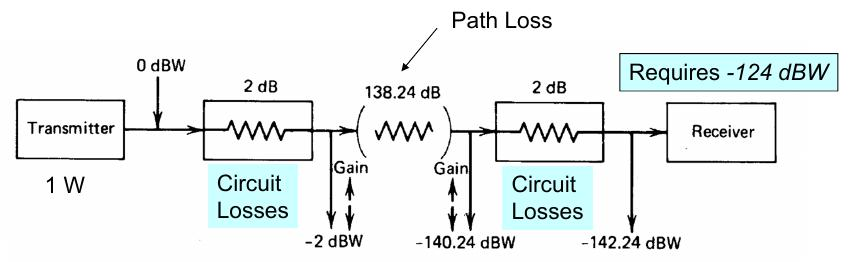
\includegraphics[scale=0.6]{linkdesign}
\end{figure}

\f{synchronisation}
\begin{itemize}
 \item signal influenced by: frequency offset, phase offset, hardware delays
 \item recievers try to:
 \begin{itemize}
  \item detach information from carrier (frequency)
  \item estimate and remove offsets
 \end{itemize}
 \item demodulation and estimation
 \item phase lock loop techniques
 \item Typical Bandwidth: 800 Hz (near-Earth), or 20 Hz (Deep-Space)
\end{itemize}

\f{system- \& error budgets}
\begin{itemize}
 \item predicting and managing variability
 \item propagete errors through a system
 \item link aspects of design and environment to capabilities and tolerances
 \item determine and track critical parameters
\end{itemize}

\f{channel encoding}
\begin{itemize}
 \item encoder takes $k$ incoming bits, maps them to $n$ outgoing bits ($n> k$)
 \item $n-k$ bits for error detection
 \item decoder does reverse process
\end{itemize}
\section{Power Generation}
\begin{itemize}
 \item individual atoms have discrete energy levels
 \item probability of occupation at energy E
 \[f(E) = \frac{1}{1+e^{\frac{E-E_F}{kT}}}\]
 \item current is conducted via electrons in the conduction band (electrons)
 \item since there are vacant positions in the valence band, the electrons there can contribute to the current as well (holes)
 \item electrons and holes are treated as quasi free particles
 \item doping of semiconductors: replace a group of atoms by a group of atoms with lower or higher ordinal number (acceptors/donors)
 \item n-doped: higher ordinal number, p-doped: lower ordinal number
 \item so far: semiconductor in equilibrium, now: under illumination
 \item energy of light is added to the electron's energy which can lift the electron from the valence band to the conduction band
 \item recombination:
 \begin{itemize}
  \item light creates electron hole pairs
  \item if light is switched off: recombination
  \item but also present: radiative recombination (cannot be prevented)
 \end{itemize}
 \item pn junction: bring p- and n- doped semiconductor in contact
 \item upon forming the junction, there is a large concentration gradient and an associated diffusion current from holes leaving the p region and e- leaving the n region
 \item at the same time, a space charge is created by the ionized dopant atoms, in the resulting electrical field an opposing drift current develops
 \item in equilibrium, both currents are equal (for e- as well as holes) and no net current flows
 \item pn-junction under illumination = solar cell
 \item Summary solar cell principles
 \begin{itemize}
  \item a semiconductor has a gap in the energy band diagram
  \item at T$>$0 free charge carriers (electrons, holes) exist
  \item by doping, one type is increased dramatically which leads to the distinction majority/minority carrier
  \item under illumination, minority carriers are created
  \item due to the fact that there is a gap in the allowed energy levels, they don’t relax immediately but have a finite lifetime $\uptau$
  \item if they can be extracted before they recombine, they provide an external current $\Rightarrow$ solar cell
  \item a pn junction does exactly that. The built-in field creates an asymmetry in the band structure. Majority carrier cannot cross it, but minority carriers can.
  \item if a charge carrier crosses the pn junction, it is transformed from a minority carrier (e.g. e- in the p doped material into a majority carrier in the n doped side) with 
  essentially infinite lifetime
 \end{itemize}
\end{itemize}

\subsection{solar cell basics}
For real solar cells, the following idealizations are not valid any more:
\begin{itemize}
 \item infinite cell dimensions: real solar cells have surfaces, which are ideal recombination sites
 \item homogeneous carrier generation G: the absorption is wavelength and depth dependent (longer wavelength has larger penetration depth)
 \item recombination in the depleted region cannot always be neglected
\end{itemize}
Typically, the I-V curves are plotted in the first quadrant. Key parameters describing the IV curve:
\begin{itemize}
 \item ppen circuit voltage $V_{oc}$
 \item short circuit current $I_{sc}$
 \item maximum power ($P_{max}$ – $V_{mp}$/$I_{Mp}$)
\end{itemize} 
\begin{figure}[!ht]
 \centering
 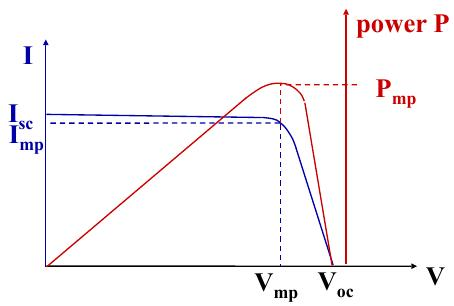
\includegraphics[scale=0.5]{solarcell}
\end{figure}

\subsection{solar cells for space}
Main requirements:
\begin{itemize}
 \item high efficiency
 \item low mass
 \item radiation resistant
\end{itemize}
Evolution: Si cells $\Rightarrow$ cells based on direct semiconductors $\Rightarrow$ multijunction cells.\\
\vspace*{3pt}

\noindent \textbf{multijunction cells}
\begin{itemize}
 \item efficiency of Si cells: 18\%
 \item additional junction reduces thermalization losses and increases efficiency $\Rightarrow$ multijunction cells
\end{itemize}
\begin{figure}[!ht]
 \centering
 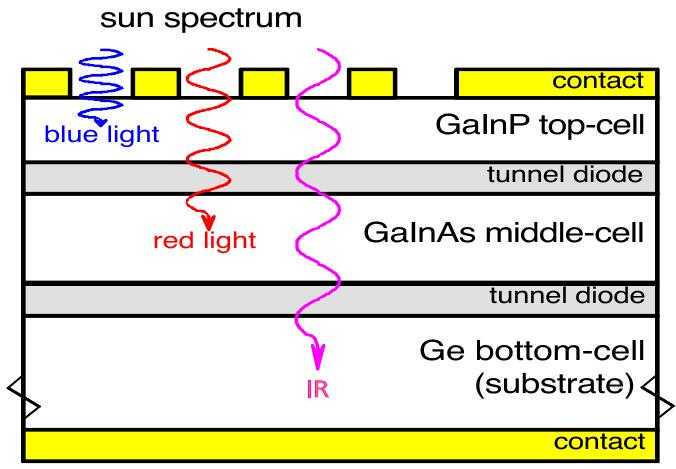
\includegraphics[scale=0.5]{triplejunction}
\end{figure}

\subsection{solar array technology}
\textbf{radiation environment in space}:
\begin{itemize}
 \item protons and electrons trapped in the earth magnetic field 
 \item solar protons 
\end{itemize}
\textbf{damage caused by particle radiation}:
\begin{itemize}
 \item ionization damage
 \item displacement damage 
\end{itemize}
\textbf{matching of solar cells}:
\[\text{current}I(S) = \sum I_{\nu}(U)\]
\[\text{voltage}V(S) = \sum V_{\mu}(I)\]
\[I(S) = n\cdot I_{cell}\]
\[V(S) = m\cdot V_{cell}\]
\textbf{power prediction}
\begin{enumerate}
 \item mission profile
 \begin{itemize}
  \item launch date
  \item launcher
  \item transfer orbits
  \item final orbit
  \item lifetime
  \item power requirements and power profile
  \item solar array orientation
 \end{itemize}
 \item satellite configuration
 \begin{itemize}
  \item power control and power conditioning (fixed voltage or maximum power tracking)
  \item solar generator type (body mounted, deployable fixed or sun oriented)
 \end{itemize}
 \item main parameters derived from orbit
 \begin{itemize}
  \item intensity and incidence angle of sun insolation over mission time
  \item effective Earth/planet radiation and albedo
  \item type, spectrum and intensity of charged particle irradiation
  \item loss factors BOM and EOM
  \item optimum solar cell and coverglass type
 \end{itemize}
\end{enumerate}
\textbf{power limiting factors} 
\vspace*{3pt}

\noindent basic and design related:
 \begin{itemize}
  \item temperature
  \item calibration inaccuracy
  \item mismatch
  \item coverglass gain/loss
  \item cable losses
  \item random failures
 \end{itemize}

\noindent mission related:
 \begin{itemize}
  \item sun intensity
  \item irradiation angle
  \item charged particles 
  \item micrometeorites/debris
 \end{itemize}
\textbf{mechanical solar array design} 
\vspace*{3pt}

\noindent so far: situation in orbit, now: mechanical criteria during satellite launch
 \begin{itemize}
  \item it has to be folded to the satellite sidewall in order to fit inside the launch vehicle
  \item it has to supply power during transfer orbit ($\rightarrow$ partial deployment)
  \item it has to be fully deployed once in geosynchronous orbit
  \item the mechanical design has to survive the acoustic loads (created by the main engines of the launch vehicle, reflected from the launch pad) and vibrational loads
 \end{itemize}

\section{Power System}
\begin{itemize}
 \item Power System Design
 \item Energy: Source and Generation
 \item Energy storage (Battery)
 \item Power Conditioning (PCU)
 \item Power Distribution (PDU)
 \item Thermal Control
 \item Reliability Aspects
\end{itemize}
\subsection{Power System Design}
\begin{itemize}
 \item supply electrical power to spacecraft loads
 \item control and distribute electrical power
 \item meet average and peak electrical loads
 \item provide power conditioning and conversion
 \item provide command and telemetry capability
 \item protect spacecraft against EPS failure
 \item suppress transient bus voltage spikes
 \item provide energy storage for eclipse and peak demands
 \item provide specialized power for specific functions such as firing ordinance for mechanism deployment
\end{itemize}
\subsection{Power System Functions}
\begin{itemize}
 \item power source (e.g. solar array, radio-isotope thermoelectric generator, nuclear reactor, primary batteries, ...)
 \item source control (regulators)
 \item power management and distribution
 \item power processors (dc/dc- or dc/ac-converters, regulators)
 \item energy storage control (charger, regulator)
 \item energy storage (batteries, flywheels)
\end{itemize}
\subsection{Power Sources}
\begin{itemize}
 \item photovoltaic: conversion of solar radiation (light) to electrical current; solar generator equipped with Silicon (Si) or Gallium-Arsenid (GaAs) cells
 \item radio-isotope thermoelectric generators
 \begin{itemize}
  \item deep space missions, military missions in low earth orbit 
  \item advantages: continuous power supply, no external supply needed, high reliability, small volume, low mass, high lifetime
  \item disadvantages: safety measures needed during launch and launch preparation, shielding necessary to protect spacecraft, regulation in case of launch failure
 \end{itemize}
\end{itemize}
\begin{figure}[!ht]
 \centering
 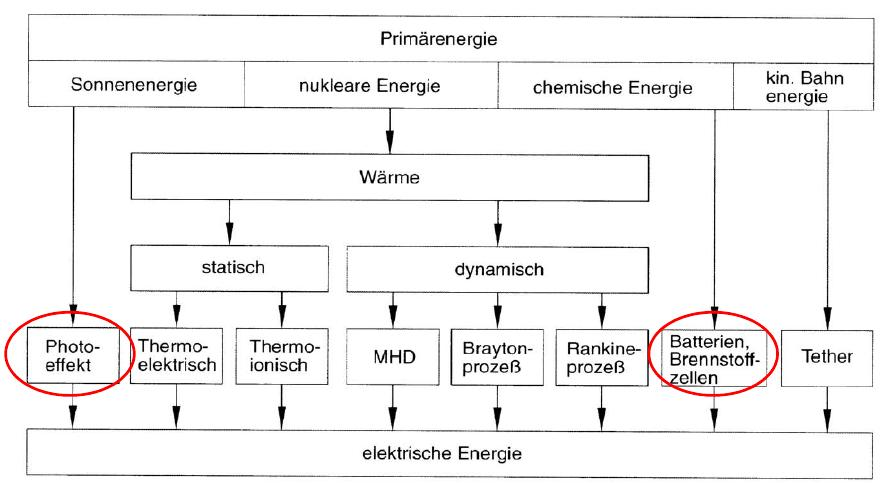
\includegraphics[scale=0.6]{energysources}
 \caption{Energy Sources}
\end{figure}
\begin{figure}[!ht]
 \centering
 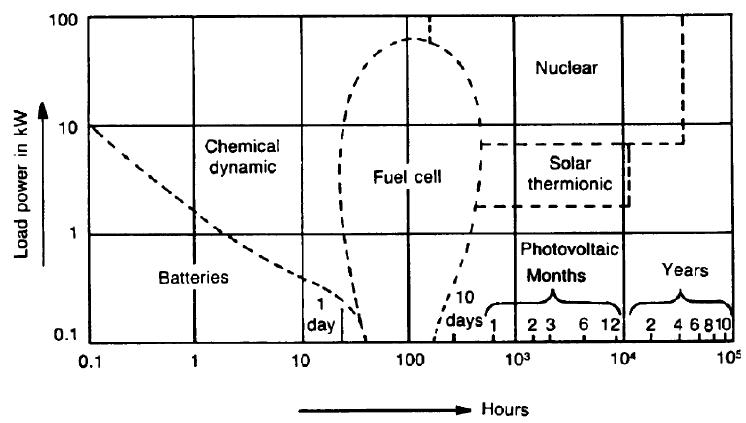
\includegraphics[scale=0.6]{energysourcesComparison}
 \caption{Comparison of Energy Sources}
\end{figure}

\subsection{Energy Storage}
 \begin{itemize}
  \item battery types: NiCD (no more used), NiH2 (mainly in telecommuniction satellites), Li-Ion (state of art), Li-Polymer (not yet used in space)
  \item fuel cells (ISS)
 \end{itemize}
\subsection{Source Control}
\begin{itemize}
 \item shunt regulator
 \item series regulator
 \item linear regulator
 \item peak power point tracker
\end{itemize}
\subsection{Main Requirements and Design Parameters}
\begin{itemize}
 \item average and peak power: determines the size of the solar array
 \item peak power: determines size of battery capacity
 \item battery charging: determines the solar array
 \item maximum discharge DoD: $< 40\%$ for Li-Ion
 \item mission lifetime: determines the degradation und subsequently sizing of battery and solar array
 \item orbit geometry: determines the available solar energy, radiation environment and eclipse durations
 \item solar constant: $1358 \frac{W}{m^2}$ mean above atmosphere. Seasonal variation: $1310-1400 \frac{W}{m^2}$
 \item satellite must be able to recover from total power loss without assistance from ground 
\end{itemize}

\subsection{Radiation Effects}
The following impacts on operation of electronic systems are associated with the charged particle environment:
\begin{itemize}
 \item TID (total ionization dose): degradation of electronics which result from proton and electron degradation in semiconductor devices
 \item SEL (single event latch-up): SELs occur when a single event causes a high current state. They may destroy the device, or they may be recoverable with a power-reset.
 \item SEB (single event burnout): heavy ion passes through a MOSFET (metal-oxide-semiconductor field-effect transistor). This induces a current flow which leads to device destruction 
 if sufficient short-circuit energy is available.
 \item SEU (single event upset): transients induced by charged particles that lose energy by ionizing the crystal lattice, leaving a wake of electron-hole pairs. The charged particles 
 usually arise from the radiation belts or from cosmic rays
\end{itemize}
\[\frac{\text{EOL}}{\text{BOL}} = \text{degradation}\]
\subsection{Efficiency and Degradation Consideration}
\begin{itemize}
 \item production efficiency $\eta$ of solar cells (14-22\%)
 \item path efficiency from solar array through batteries to loads: $X_e=0.65, X_d=0.85$ (direct energy transfer), $X_e=0.60, X_d=0.80$ (peak power tracking)
 \item inherent degradation: $I_d \approx 0.77$, ranges from $0.49-0.88$
 \item cosine loss, angle $\Theta$ between array normal and sun vector; typically use worst-case sun-angle
 \item life degradation: micrometeorites, radiation, etc. (2-4\% per year)\[L_d = (1-\text{degradation per year})^{\text{satellite life}}\]
\end{itemize}
\subsection{From Begin of Life to End of Life}
\[P_{o} = \eta\cdot 1358\frac{W}{m^2} \text{\qquad output power}\]
\[P_{BOL} = P_o\cdot I_d\cdot cos(\Theta)\]
\[P_{EOL} = L_d\cdot P_{BOL}\]
solar array size to meet power requirement:
\[A_{sa} = \frac{P_{sa}}{P_{EOL}}\]
mass of solar array ranges from $14$ to $47 \frac{W}{kg}$:
\[M_{sa} = 0.04\cdot P_{sa} \text{ \qquad (for } 25 \frac{W}{kg})\]
\subsection{Maximum Power Point Tracker (MPPT)}
\begin{itemize}
 \item continuously measures the power from the solar array and determines the maximum power point 
 \item adjusts the solar array interface voltage such that the actual power demand of the spacecraft can be delivered
 \item maximum efficiency ($>99\%$) can be achieved when the solar array interface voltage is close to the battery voltage
\end{itemize}
\subsection{Pros and Cons of Power Regulation}
\begin{itemize}
 \item power damper: excessive power will be absorbed in high power resistors, switch control system for resistors $\Rightarrow$ impact on thermal control system, as significant power 
 dissipation occurs 
 \item linear regulator: excessive power will be absorbed in high power transistor $\Rightarrow$ impact on thermal control system, as significant power dissipation occurs 
 \item shunt regulator: simple, robust, failsafe $\Rightarrow$ requires high number of cells per string to ensure battery charging and minimum power 
 \item MPPT: highest efficiency and minimum solar array size, complex in redundancy concept, each wing requires a dedicated MPPT
\end{itemize}
\subsection{Battery Sizing}
Power need:
\[P_{avg} = V_{bus}\cdot I\]
\[Ah_{avg} = \frac{T_e}{1h}\cdot I\]
\[Ah_{total} = \frac{Ah_{avg}}{DoD}\]
Capacity:
\[C_r = \frac{P_{avg}\cdot T_e}{DoD\cdot N_{bat} \cdot \eta}\]
\subsection{Power Distribution}
\begin{itemize}
 \item protection by fuse
 \item electronic protections
 \item limit current in failure case
 \item isolate failed components from bus
\end{itemize}

\section{Thermal Testing}
\section{Spacecraft Operations}
\begin{itemize}
 \item remotely control of a spacecraft
 \item after the separation from the launcher the satellite can only be controlled remotely
 \item the operations phase shows ultimately if all considerations in the development phase were right and the mission is successful
 \item especially at the early operations phase and in critical situations the public interest is large and the fascination of space missions is noticeable
 \item at this moment, mission operations is in focus and it is decided whether the mission is successful or not
 \item mission objectives determine all aspects of a space mission, including the operations. All mission and system requirements are derived either from these objectives or mission
 constraints.
\end{itemize}
\f{Basic Functions of Spacecraft Operations}
\begin{itemize}
 \item mission planning
 \begin{itemize}
  \item priorization of user requests
  \item development of timelines for operations
  \item development of timelines for ground stations
  \item creation of command files
  \item support of special requests
  \item computation of orbital elements
  \item operation and use of ground data networks
  \item optimization of utilization
 \end{itemize}

 \item training of personnel
 \begin{itemize}
  \item development of a training program
  \item training on a simulator
  \item training on spacecraft
  \item continuous training (in flight)
 \end{itemize}

 \item mission operations
 \begin{itemize}
  \item commanding of spacecraft
  \item monitoring of subsystems (online)
  \item payload management
  \item trend analysis (offline)
  \item anomaly handling
 \end{itemize}

 \item scientific and technical support 
 \begin{itemize}
  \item support in both directions (operations $\leftrightarrow$ development)
  \item early start of contributions (already at study level in Phase A)
  \item construction and test
  \item planning of orbital maneuvers
  \item management of payload and subsystems
  \item anomaly management
  \item flight software management
  \item management of simulators
  \item database management
  \item trend analysis for the spacecraft
 \end{itemize}

\end{itemize}

\end{document}
